\documentclass{beamer}
\usetheme{Warsaw}
\usepackage{natbib}
\usepackage{graphicx}
% ------------------------------------------------------------------------
% Packages
% ------------------------------------------------------------------------
\usepackage{amsmath}

% ------------------------------------------------------------------------
% Macros
% ------------------------------------------------------------------------
%~~~~~~~~~~~~~~~
% List shorthand
%~~~~~~~~~~~~~~~
\newcommand{\BIT}{\begin{itemize}}
\newcommand{\EIT}{\end{itemize}}
\newcommand{\BNUM}{\begin{enumerate}}
\newcommand{\ENUM}{\end{enumerate}}
%~~~~~~~~~~~~~~~
% Text with quads around it
%~~~~~~~~~~~~~~~
\newcommand{\qtext}[1]{\quad\text{#1}\quad}
%~~~~~~~~~~~~~~~
% Shorthand for math formatting
%~~~~~~~~~~~~~~~
\newcommand\mbb[1]{\mathbb{#1}}
\newcommand\mbf[1]{\mathbf{#1}}
\def\mc#1{\mathcal{#1}}
\def\mrm#1{\mathrm{#1}}
%~~~~~~~~~~~~~~~
% Common sets
%~~~~~~~~~~~~~~~
\def\reals{\mathbb{R}} % Real number symbol
\def\integers{\mathbb{Z}} % Integer symbol
\def\rationals{\mathbb{Q}} % Rational numbers
\def\naturals{\mathbb{N}} % Natural numbers
\def\complex{\mathbb{C}} % Complex numbers
\def\simplex{\mathcal{S}} % Simplex
%~~~~~~~~~~~~~~~
% Common functions
%~~~~~~~~~~~~~~~
\renewcommand{\exp}[1]{\operatorname{exp}\left(#1\right)} % Exponential
\def\indic#1{\mbb{I}\left({#1}\right)} % Indicator function
\providecommand{\argmax}{\mathop\mathrm{arg max}} % Defining math symbols
\providecommand{\argmin}{\mathop\mathrm{arg min}}
\providecommand{\arccos}{\mathop\mathrm{arccos}}
\providecommand{\asinh}{\mathop\mathrm{asinh}}
\providecommand{\dom}{\mathop\mathrm{dom}} % Domain
\providecommand{\range}{\mathop\mathrm{range}} % Range
\providecommand{\diag}{\mathop\mathrm{diag}}
\providecommand{\tr}{\mathop\mathrm{tr}}
\providecommand{\abs}{\mathop\mathrm{abs}}
\providecommand{\card}{\mathop\mathrm{card}}
\providecommand{\sign}{\mathop\mathrm{sign}}
\def\rank#1{\mathrm{rank}({#1})}
\def\supp#1{\mathrm{supp}({#1})}
%~~~~~~~~~~~~~~~
% Common probability symbols
%~~~~~~~~~~~~~~~
\def\E{\mathbb{E}} % Expectation symbol
\def\Earg#1{\E\left[{#1}\right]}
\def\Esubarg#1#2{\E_{#1}\left[{#2}\right]}
\def\P{\mathbb{P}} % Probability symbol
\def\Parg#1{\P\left({#1}\right)}
\def\Psubarg#1#2{\P_{#1}\left[{#2}\right]}
\def\Cov{\mrm{Cov}} % Covariance symbol
\def\Covarg#1{\Cov\left[{#1}\right]}
\def\Covsubarg#1#2{\Cov_{#1}\left[{#2}\right]}
\def\Var{\mrm{Var}}
\def\Vararg#1{\Var\left(#1\right)}
\def\Varsubarg#1#2{\Var_{#1}\left(#2\right)}
\newcommand{\family}{\mathcal{P}} % probability family
\newcommand{\eps}{\epsilon}
\def\absarg#1{\left|#1\right|}
\def\msarg#1{\left(#1\right)^{2}}
\def\logarg#1{\log\left(#1\right)}
%~~~~~~~~~~~~~~~
% Distributions
%~~~~~~~~~~~~~~~
\def\Gsn{\mathcal{N}}
\def\Ber{\textnormal{Ber}}
\def\Bin{\textnormal{Bin}}
\def\Unif{\textnormal{Unif}}
\def\Mult{\textnormal{Mult}}
\def\Cat{\textnormal{Cat}}
\def\Gam{\textnormal{Gam}}
\def\InvGam{\textnormal{InvGam}}
\def\NegMult{\textnormal{NegMult}}
\def\Dir{\textnormal{Dir}}
\def\Lap{\textnormal{Laplace}}
\def\Bet{\textnormal{Beta}}
\def\Poi{\textnormal{Poi}}
\def\HypGeo{\textnormal{HypGeo}}
\def\GEM{\textnormal{GEM}}
\def\BP{\textnormal{BP}}
\def\DP{\textnormal{DP}}
\def\BeP{\textnormal{BeP}}
%~~~~~~~~~~~~~~~
% Theorem-like environments
%~~~~~~~~~~~~~~~

%-----------------------
% Probability sets
%-----------------------
\newcommand{\X}{\mathcal{X}}
\newcommand{\Y}{\mathcal{Y}}
\newcommand{\D}{\mathcal{D}}
\newcommand{\Scal}{\mathcal{S}}
%-----------------------
% vector notation
%-----------------------
\newcommand{\bx}{\mathbf{x}}
\newcommand{\by}{\mathbf{y}}
\newcommand{\bt}{\mathbf{t}}
\newcommand{\xbar}{\overline{x}}
\newcommand{\Xbar}{\overline{X}}
\newcommand{\tolaw}{\xrightarrow{\mathcal{L}}}
\newcommand{\toprob}{\xrightarrow{\mathbb{P}}}
\newcommand{\laweq}{\overset{\mathcal{L}}{=}}
\newcommand{\F}{\mathcal{F}}
\def\colarg#1#2{\textcolor[HTML]{#1}{#2}}

\setbeamersize{text margin left=5pt,text margin right=5pt}

\setbeamerfont{institute}{size=\fontsize{7pt}{8pt}}
\setbeamerfont{date}{size=\fontsize{0pt}{0pt}}

\title{Methods for Regime Detection and Multitable Analysis}
\author{Kris Sankaran}

\begin{document}
\maketitle

\begin{frame}
  \frametitle{Problems of Interest}
 \begin{itemize}
 \item Regime Detection: Can we segment time intervals in a microbiome study in
   an unsupervised way?
   \begin{itemize}
   \item Intervals with similar dynamics should be placed in the same regime
   \item Can we characterize differences between taxa during these regimes?
   \end{itemize}
 \item Multitable Analysis: How should we simultaneously study multiple
   measurement types?
   \begin{itemize}
   \item How do different measurement types covary with one another?
   \item Compared to usual regression, when there are multiple related
     responses, there are fewer obvious practical approaches
   \end{itemize}
 \item Philosophy: Distill relevant themes, provide concrete workflows, and
   systematize data / study specific recommendations
 \end{itemize} 
\end{frame}

\section{Regime Detection}
\label{sec:regime_detection}

\begin{frame}
  \frametitle{Recap}
 \begin{itemize}
 \item For this case study, we again use the antibiotics data of
   \citep{dethlefsen2008pervasive}
   \begin{itemize}
   \item 3 subjects at between 52 and 56 timepoints
   \item Two antibiotic time courses introduced around 12 - 16 and 40 - 44
   \item Long term effects in Subject F previously observed
   \end{itemize} 
 \item Last time we approached the regime detection problem using hierarchical
   clustering with various distances, HMMs, Sticky HMMs, Infinite HMMs, and
   Switching Dynamical Systems
 \item We continue that survey using different approaches
 \end{itemize} 
\end{frame}

\begin{frame}
  \frametitle{CART}
  \begin{itemize}
  \item Order species according to a hierarchical
    clustering\footnote{Alternatively, use phylogenetic similarity.}, and
    consider the surface of species abundances across the time by species space
  \item CART can approximate this surface, providing a partition of timepoints
    and species in the process.
  \item Can be extended to binary data
  \item Limitation: Cannot update the species order (though you could imagine an
    iterative approach...)
  \end{itemize}  
\end{frame}

\begin{frame}
  \frametitle{CART}
\begin{itemize}
\item Structural model: The class of functions $\mathcal{F}$ that can be
  expressed as
\begin{align*}
  f\left(x\right) &= \sum_{m = 1}^{M} c_{m} \indic{x \in R_{m}},
\end{align*}
\item Fitting criteria: Minimize the expected generalization squared-error,
\begin{align*}
  \frac{1}{n} \sum_{i = 1}^{n} \left(y_{i} - c\left(x_{i}\right)\right)^{2},
\end{align*}
\item Estimation strategy: Recursively split rectangles into left ($l$) and
  right ($r$) subrectangles according to
\begin{align*}
  \left(j^{\ast}, t_{j1}^{\ast}\right) &= \arg \min_{\substack{j = 1, \dots, p \\ t_{j1} \in \reals}} \sum_{i \in R_{1, l}} \left(y_{i} - \bar{y}_{l}\right)^{2} + \sum_{i \in R_{1, r}} \left(y_{i} - \bar{y}_{r}\right)^{2}
\end{align*}
and prune to prevent overfitting
\end{itemize}
\end{frame}

\begin{frame}
  \frametitle{CART ($\asinh$ abundance)}
  \begin{figure}[ht]
    \centering
    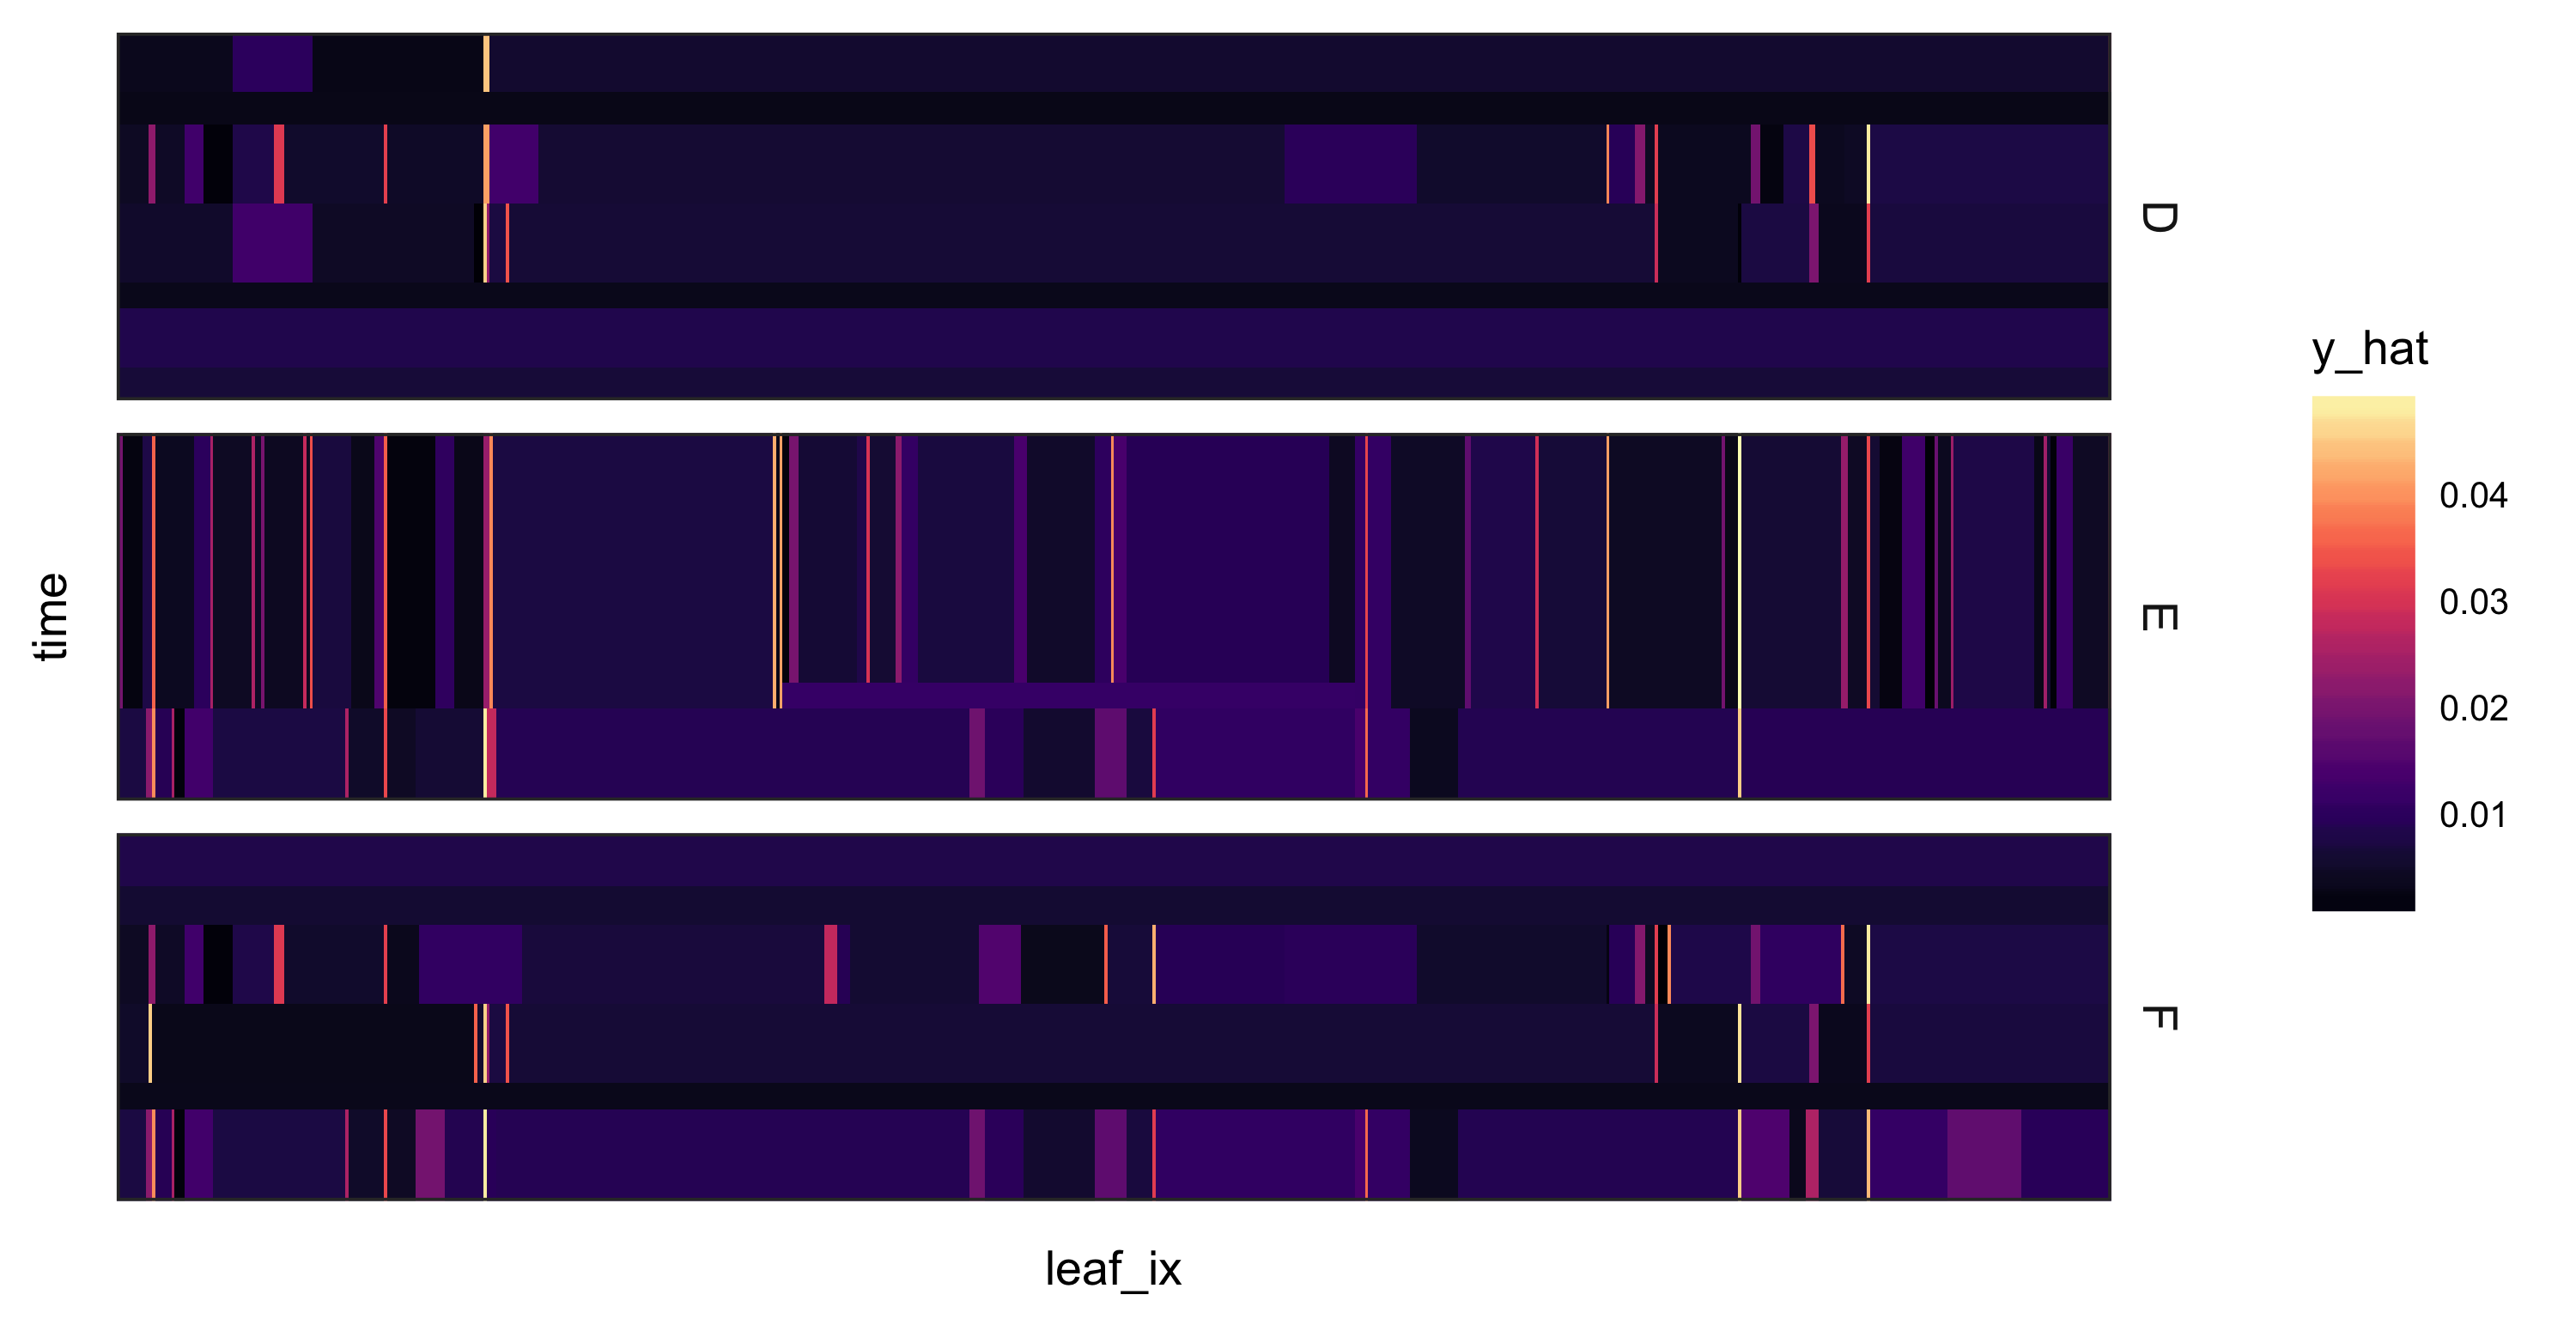
\includegraphics[width=.8\textwidth]{figure/rpart_complex_2}
    \caption{Each panel represents a subject, the $x$-axis are individual
      species, the $y$-axis indexes time, and the color is the predicted
      abundance according to CART. Note the low abundance predictions during the
      antibiotic time course. \label{fig:rpart_complex} }
  \end{figure}
\end{frame}

\begin{frame}
  \frametitle{CART (Residual)}
  \begin{figure}[ht]
    \centering
    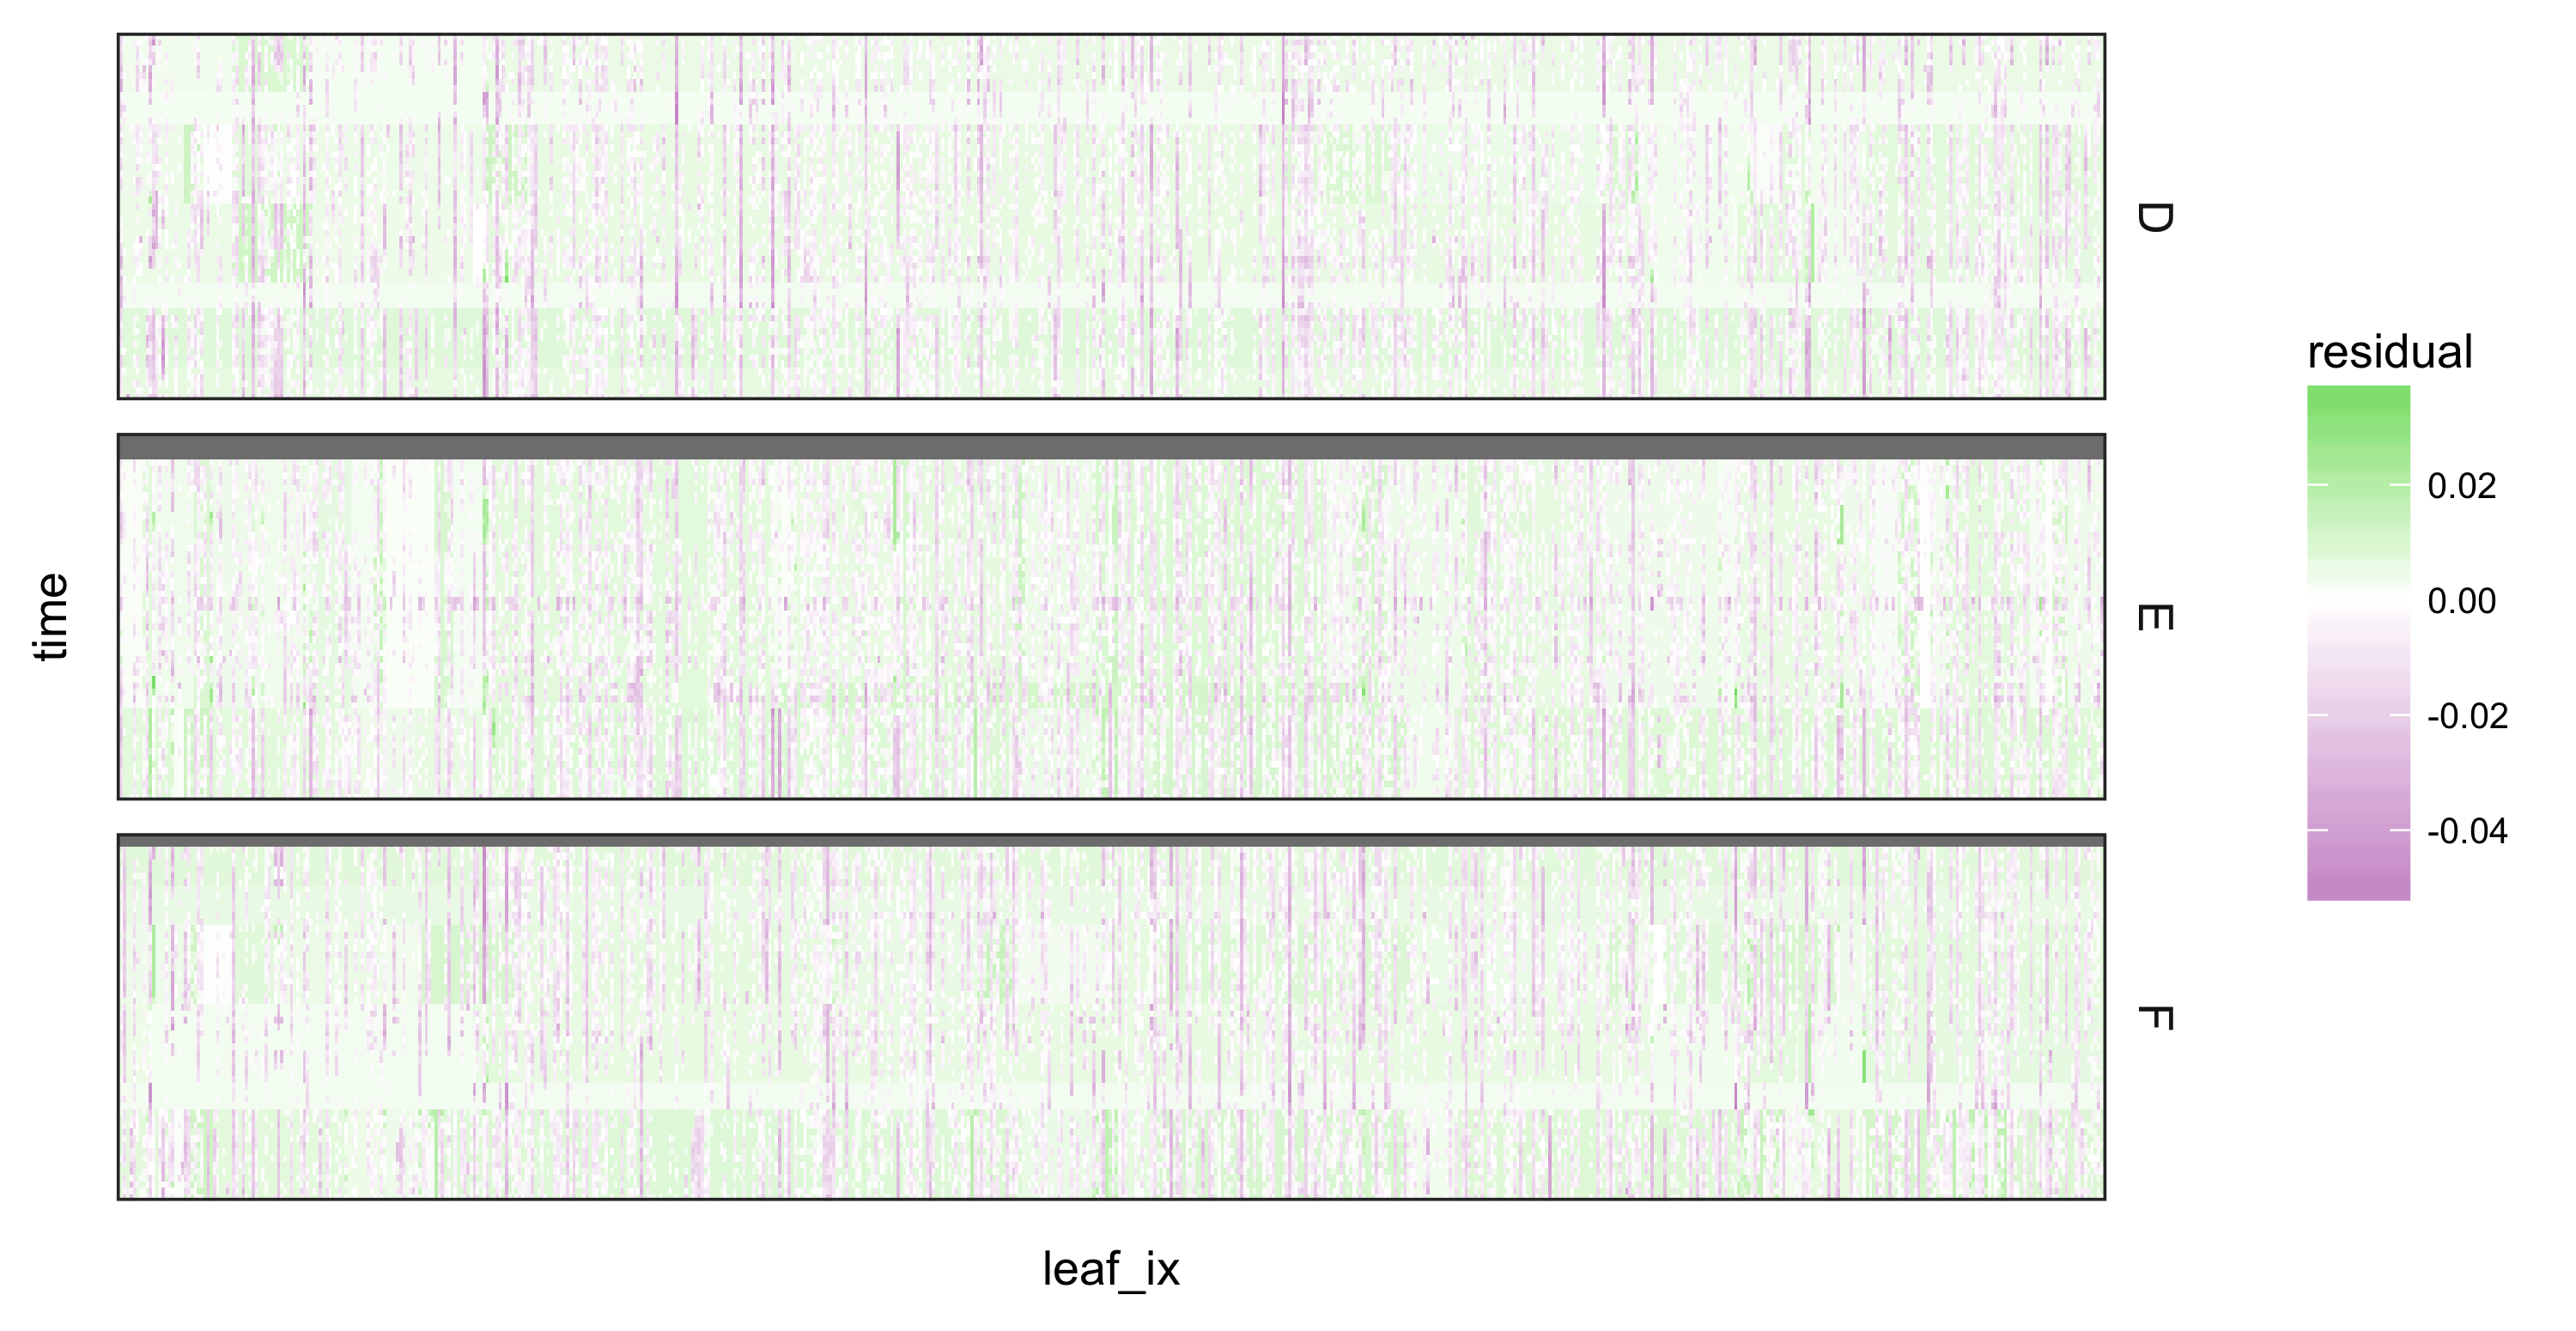
\includegraphics[width=.8\textwidth]{figure/rpart_complex_2_resid}
    \caption{An advantage of using a regression model is that we can directly
      inspect the quality of model fit, using
      residuals. \label{fig:rpart_complex_resid} }
  \end{figure}
\end{frame}

\begin{frame}
  \frametitle{Adjusting Model Complexity}
  \begin{figure}[ht]
    \centering
    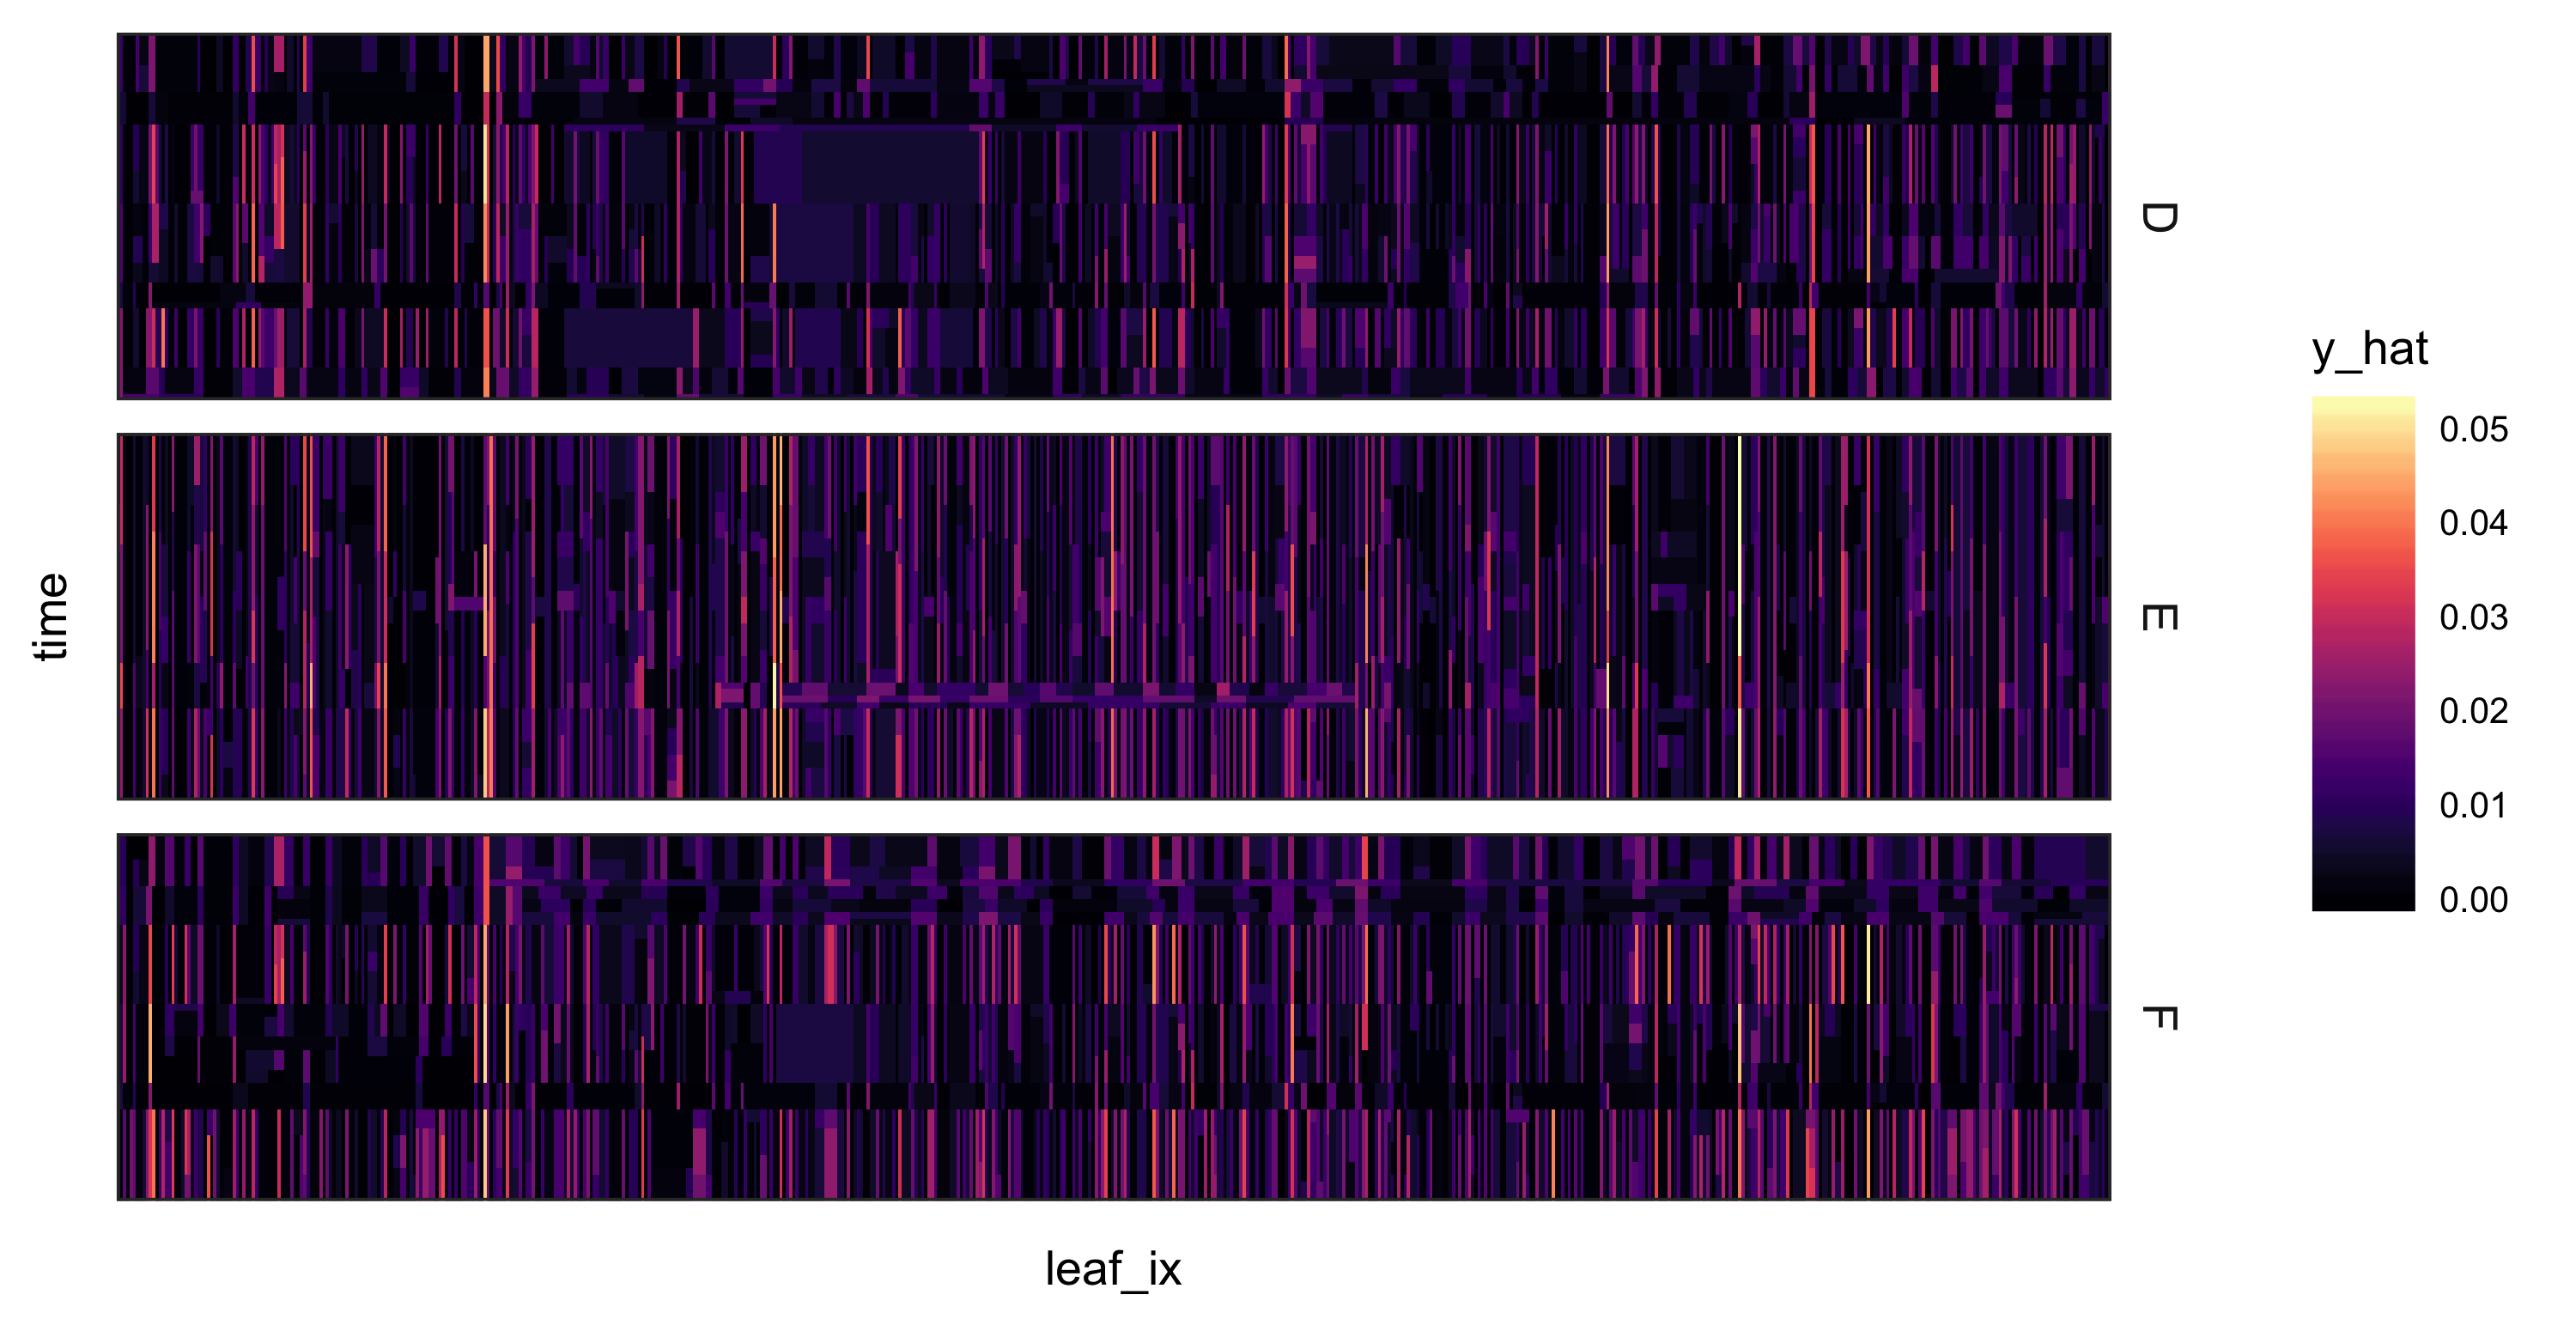
\includegraphics[width=.8\textwidth]{figure/rpart_simple}
    \caption{By increasing the model complexity, we notice species with
      increasing abundances during the antibiotic time
      courses. \label{fig:rpart_simple} }
  \end{figure}
\end{frame}


\begin{frame}
  \frametitle{CART (Presence / Absence)}
  \begin{figure}[ht]
    \centering
    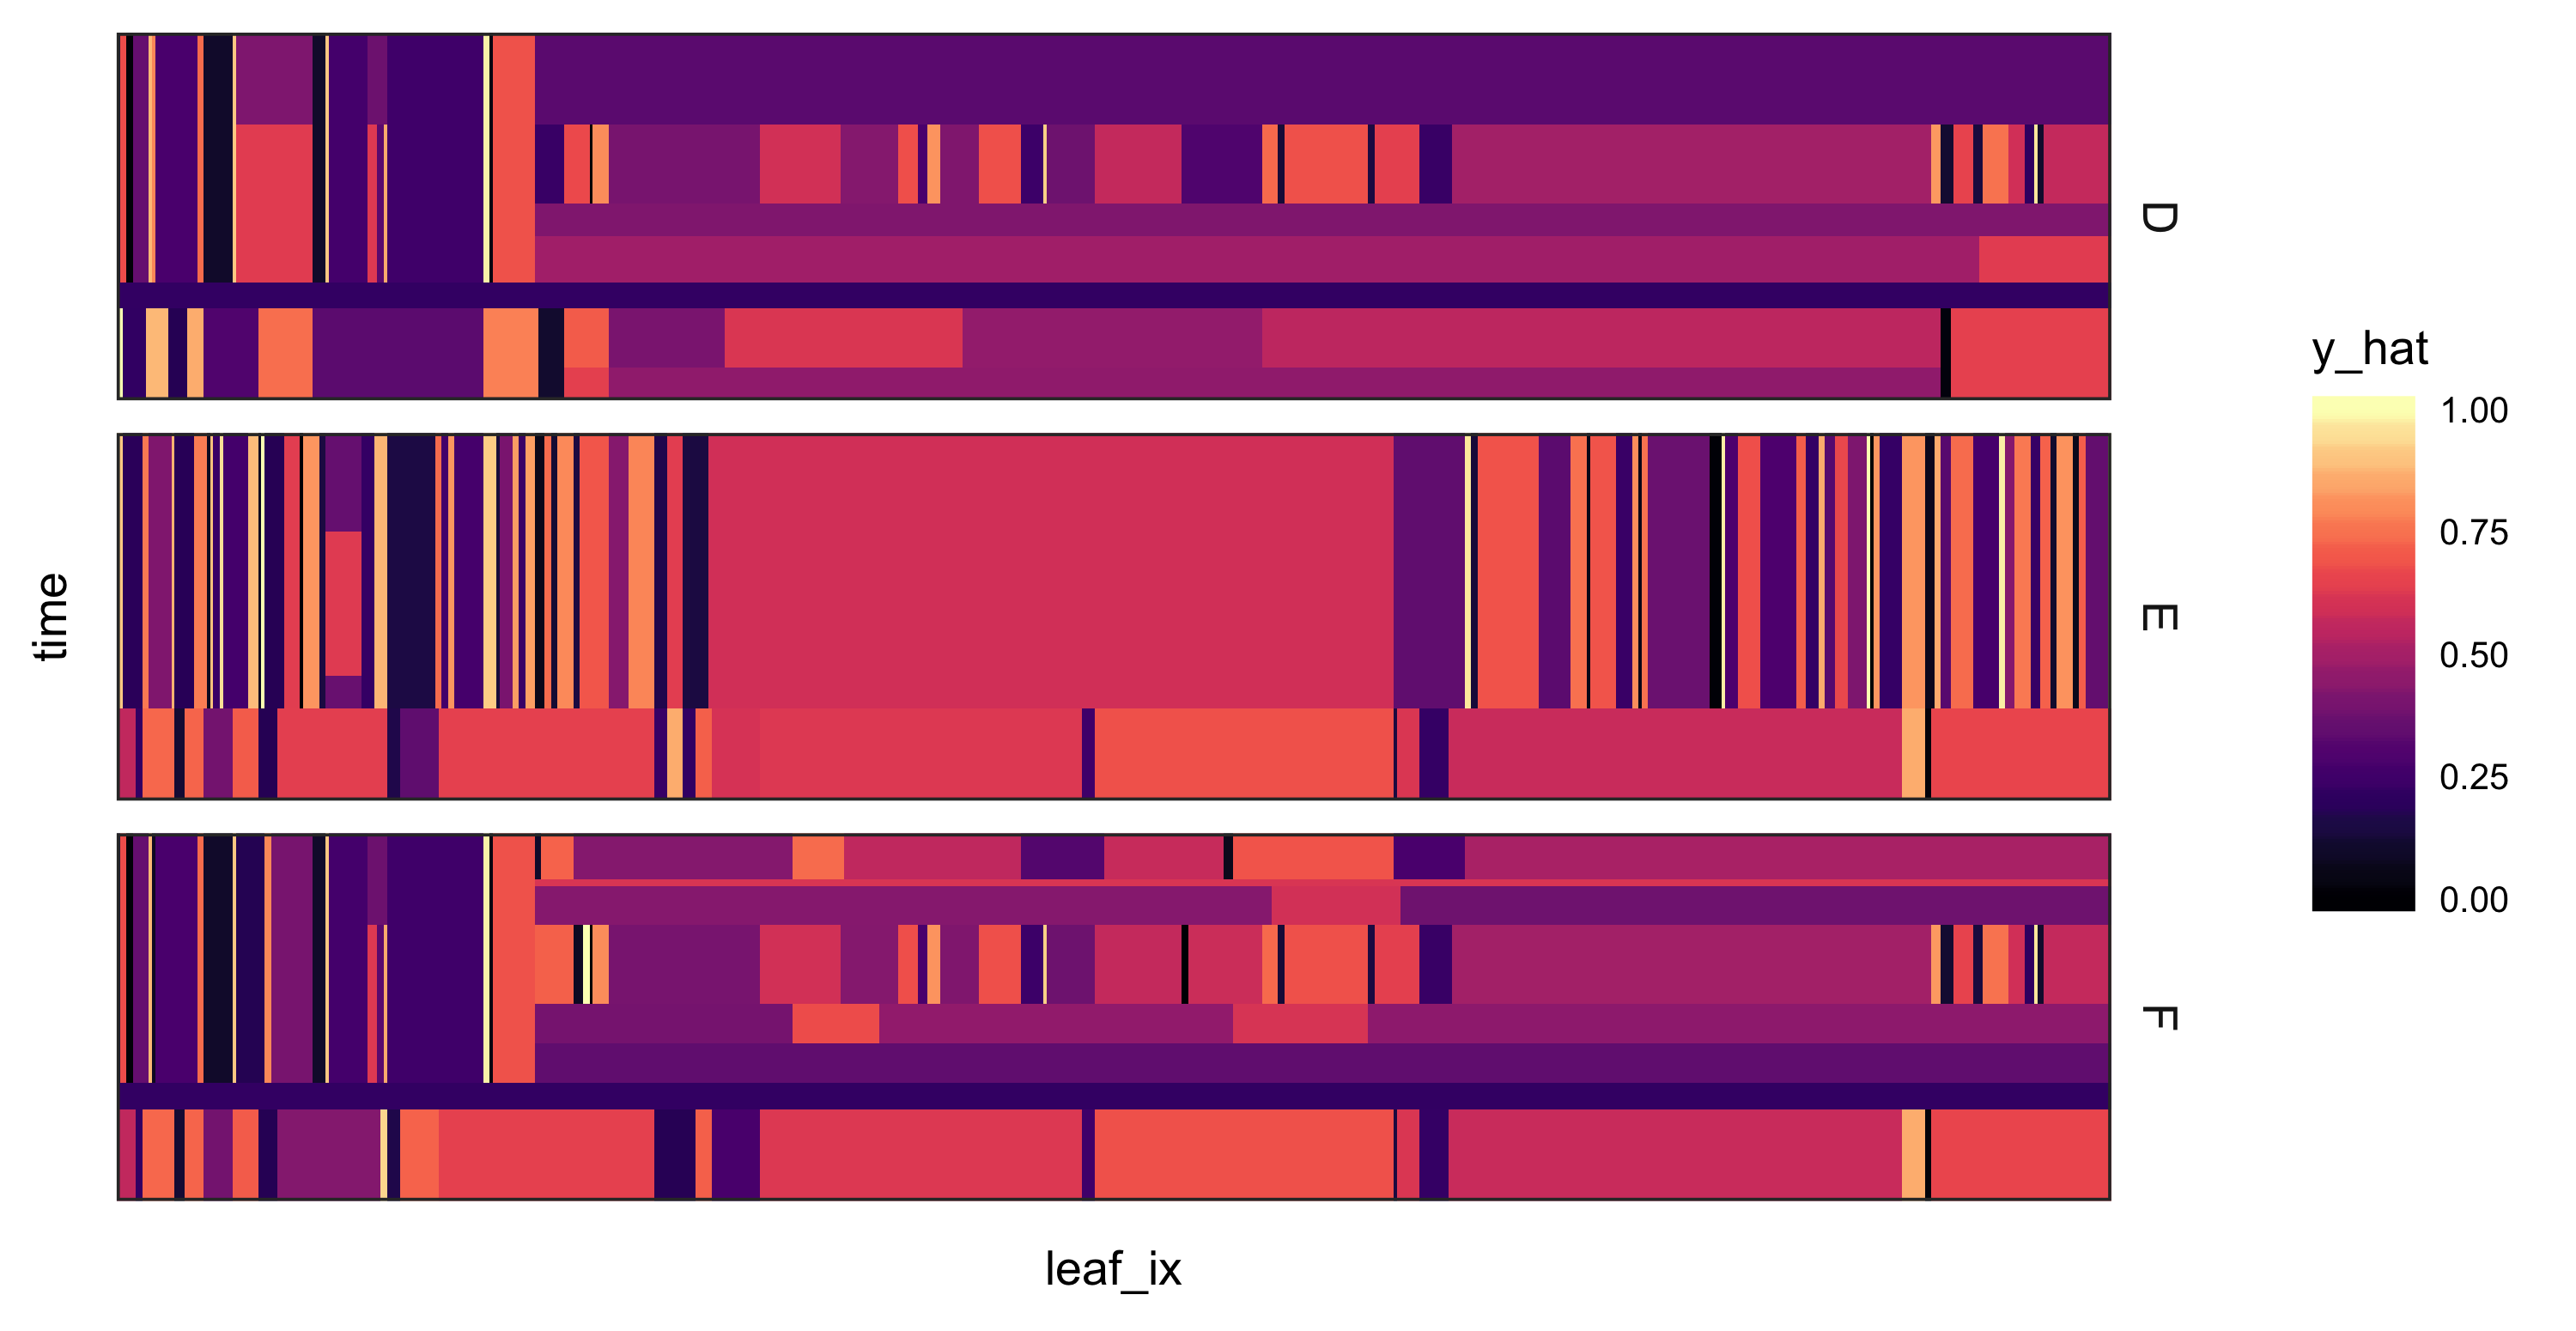
\includegraphics[width=.8\textwidth]{figure/rpart_binary}
    \caption{We can use the same method on presence-absence data, to identify
      whether certain regimes have many more exact zeros than others.
      \label{fig:rpart_binary} }
  \end{figure}
\end{frame}

\begin{frame}
  \frametitle{Aside: Sparse Time Series}
\begin{figure}[ht]
  \centering
  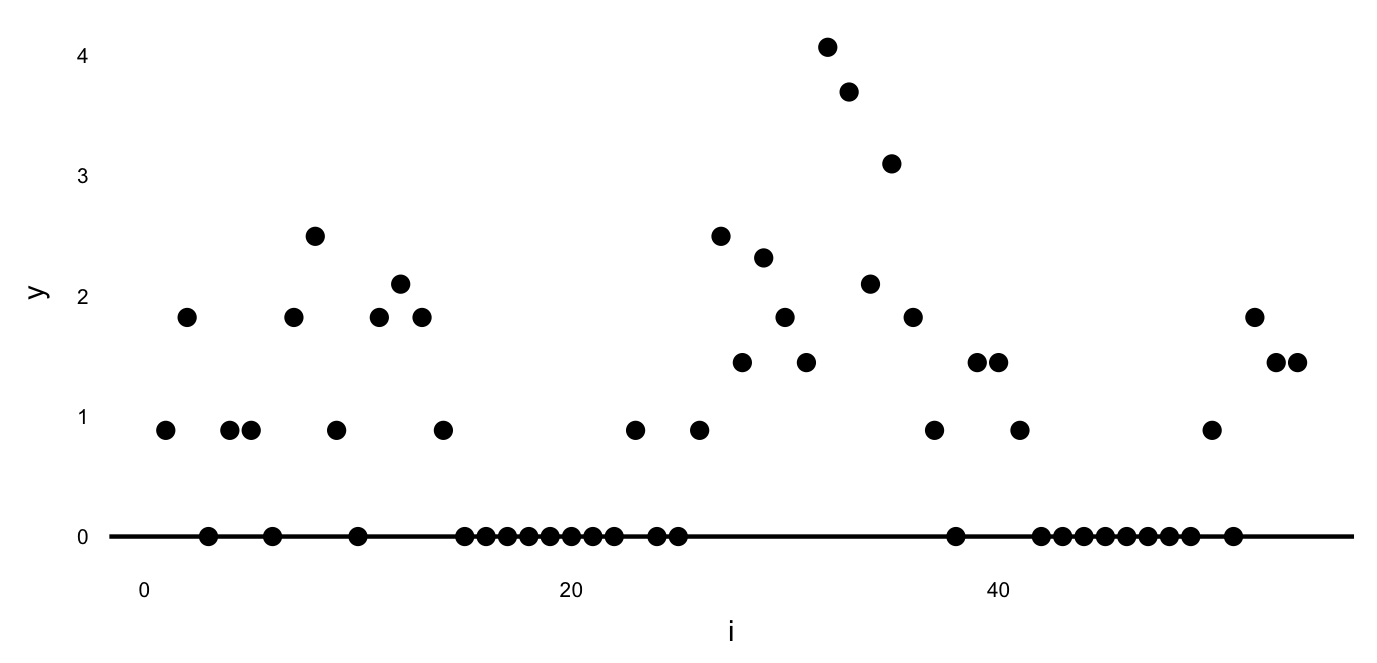
\includegraphics[width=0.9\textwidth]{figure/abt_zeros}
  \caption{One species from the antibiotics data set. It appears to have
    disappeared during the two antibiotics time courses. There is potentially
    value in modeling sequences of exact zeros in some regimes.
    \label{fig:abt_zeros} }
\end{figure}

\end{frame}

\begin{frame}
  \frametitle{Dynamic Tobit Model}
  \begin{itemize}
  \item To model sparsity in microbiome abundances, we can adopt a censoring
    point of view
  \item For example, the Dynamic Tobit model adds an extra layer of censoring on
    top of the ordinary state space model,
    \begin{align*}
      x_{t} &= Ax_{t - 1} + w_{t} \\
      \tilde{y}_{t} &= Cx_{t} + \eps_{t} \\
      y_{t} &= \tilde{y}_{t} \indic{\tilde{y}_{t} \geq c},
    \end{align*}
    where both $x$ and $\tilde{y}$ are unobserved.
  \item MCMC \citep{de1997scan, brockwell2006long, manrique1998simulation} and
    particle filtering \citep{andrieu2002particle} approaches are available
  \item Note this does not share information across species
  \end{itemize}
\end{frame}

\begin{figure}
  \frametitle{Antibiotics Example}
  \centering
  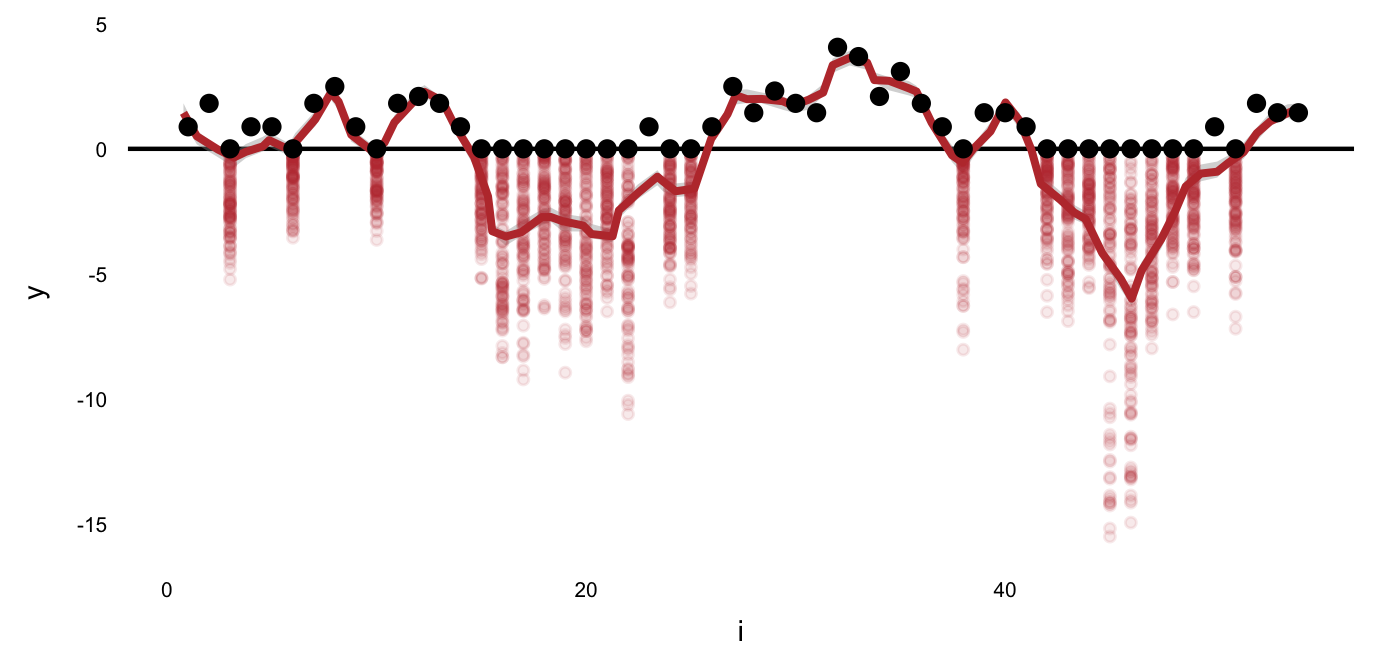
\includegraphics[width=\textwidth]{figure/abt_scan}
  \caption{Results of the scan sampler for a single species. Black points are
    observed data, red points are posterior samples, and the red line is a
    kernel smooth over samples. Implementation at
    \url{https://github.com/krisrs1128/readings/} \label{fig:abt_scan}
  }
\end{figure}

\begin{frame}
  \frametitle{Mixture of GPs}
 \begin{itemize}
 \item 
 \end{itemize} 
\end{frame}

\begin{frame}
  \frametitle{Mixture of GPs}
\end{frame}

\begin{frame}
  \frametitle{Changepoint Detection}
\end{frame}

\begin{frame}
  \frametitle{Changepoint Detection}
\end{frame}

\section{Multitable Analysis}
\label{sec:multitable analysis}

\begin{frame}
  \frametitle{WELL-China Study}
  \begin{itemize}
  \item Focused on the relationship between various indicators of wellness.
  \item Data about exercise, sleep, diet, mental health for 1969 people, in
    addition to 16s data on 221 participants (with plans for metabolomics,
    methylation, ...)
  \item We focus on question of body composition vs. microbiome structure
  \end{itemize}
\end{frame}

\begin{frame}
  \frametitle{Body Composition}
  \begin{itemize}
  \item Scans from DXA sensor to provide richer information than BMI alone
  \item Can we reproduce findings relating microbiome and BMI / metabolic
    syndrome, but using our richer data on body type?
    \begin{itemize}
    \item People with similar BMI might have different disease dispositions
      depending on the distribution of lean and fat mass
    \end{itemize}
  \end{itemize}  
\end{frame}

\begin{frame}
  \frametitle{PCA}
  
\end{frame}

\begin{frame}
  \frametitle{CCA}
\end{frame}

\begin{frame}
  \frametitle{Sparse CCA}
\end{frame}

\begin{frame}
  \frametitle{Probabilistic CCA}
\end{frame}

\begin{frame}
  \frametitle{CCA + LDA}
\end{frame}

\begin{frame}
  \frametitle{Conclusion}
  
\end{frame}
\bibliographystyle{plainnat}
\bibliography{refs.bib}

\section{Testing using Distances}
\label{sec:testing_distances}

\end{document}
